\PassOptionsToPackage{unicode=true}{hyperref} % options for packages loaded elsewhere
\PassOptionsToPackage{hyphens}{url}
%
\documentclass[]{article}
\usepackage{lmodern}
\usepackage{amssymb,amsmath}
\usepackage{ifxetex,ifluatex}
\usepackage{fixltx2e} % provides \textsubscript
\ifnum 0\ifxetex 1\fi\ifluatex 1\fi=0 % if pdftex
  \usepackage[T1]{fontenc}
  \usepackage[utf8]{inputenc}
  \usepackage{textcomp} % provides euro and other symbols
\else % if luatex or xelatex
  \usepackage{unicode-math}
  \defaultfontfeatures{Ligatures=TeX,Scale=MatchLowercase}
\fi
% use upquote if available, for straight quotes in verbatim environments
\IfFileExists{upquote.sty}{\usepackage{upquote}}{}
% use microtype if available
\IfFileExists{microtype.sty}{%
\usepackage[]{microtype}
\UseMicrotypeSet[protrusion]{basicmath} % disable protrusion for tt fonts
}{}
\IfFileExists{parskip.sty}{%
\usepackage{parskip}
}{% else
\setlength{\parindent}{0pt}
\setlength{\parskip}{6pt plus 2pt minus 1pt}
}
\usepackage{hyperref}
\hypersetup{
            pdfborder={0 0 0},
            breaklinks=true}
\urlstyle{same}  % don't use monospace font for urls
\usepackage{graphicx,grffile}
\makeatletter
\def\maxwidth{\ifdim\Gin@nat@width>\linewidth\linewidth\else\Gin@nat@width\fi}
\def\maxheight{\ifdim\Gin@nat@height>\textheight\textheight\else\Gin@nat@height\fi}
\makeatother
% Scale images if necessary, so that they will not overflow the page
% margins by default, and it is still possible to overwrite the defaults
% using explicit options in \includegraphics[width, height, ...]{}
\setkeys{Gin}{width=\maxwidth,height=\maxheight,keepaspectratio}
\setlength{\emergencystretch}{3em}  % prevent overfull lines
\providecommand{\tightlist}{%
  \setlength{\itemsep}{0pt}\setlength{\parskip}{0pt}}
\setcounter{secnumdepth}{0}
% Redefines (sub)paragraphs to behave more like sections
\ifx\paragraph\undefined\else
\let\oldparagraph\paragraph
\renewcommand{\paragraph}[1]{\oldparagraph{#1}\mbox{}}
\fi
\ifx\subparagraph\undefined\else
\let\oldsubparagraph\subparagraph
\renewcommand{\subparagraph}[1]{\oldsubparagraph{#1}\mbox{}}
\fi

% set default figure placement to htbp
\makeatletter
\def\fps@figure{htbp}
\makeatother


\date{}

\begin{document}

\hypertarget{network-security}{%
\section{Network Security}\label{network-security}}

\textbf{Network Security Threats:}

\begin{itemize}
\item
  Intrusions - Unwanted access to a system
\item
  Blocking - DoS
\item
  Malware
\end{itemize}

\textbf{Domain Name System:}

DNS will resolve an IP address from a given URL by parsing the
name-server tree until it finds the given domain name. The name server
then transmits the IP address back to the client. It is unencrypted and
easily monitored.

\textbf{Threats to DNS:}

\begin{itemize}
\item
  Corrupted host platforms
\item
  Resolvers that leak queries
\item
  Name-servers that leak queries
\item
  DNS Hijacking
\item
  DNS Cache poisoning - Changing entries in a DNS table in order to
  redirect queries to fake websites (It can be used for censorship)
\item
  DNS Amplification Attack (Smurf) - A single node sends a request to a
  router, the router forwards this request to all its connected devices,
  and the devices then all send their responses to a single node which
  will cause DoS.
\end{itemize}

\textbf{DNS Protection:}

\begin{itemize}
\item
  DoT (DNS over TLS) - The first DNS encryption solution, DNS channels
  the original clients request through TLS on port 853. A secure channel
  is established with the DNS resolver.
\item
  DoH - Sends DNS requests over HTTPS
\end{itemize}

\textbf{HTTP:}

HTTP is a symmetric request-response client-server protocol. It uses
TCP.

\textbf{HTTP Session Hijacking:}

\begin{enumerate}
\def\labelenumi{\arabic{enumi}.}
\item
  Hijacker injects malicious script into the web server
\item
  The victim authenticates on the server
\item
  The server returns the page with injected script
\item
  The victim's browser executes the script and sends session cookies to
  the attacker
\item
  The attacker hijacks the user session
\end{enumerate}

\textbf{Session Side-Jacking:}

Using packet sniffing, attackers monitor session traffic and intercept
cookies after the user has authenticated with the server. If the website
only uses SSL/TLS encryption for login pages and not for the entire
session the hijacker can use the sniffed session ID to hijack the
session. The hijacker needs access to the victim's network. Using HTTPS
can prevent this as it will encrypt all traffic over HTTP.

\textbf{TCP Session Hijacking:}

When the attacker is on the same network as the client, the attacker can
sniff TCP packets and know the ACK/SEQ numbers. Attackers can then
inject a packet with the correct ACK/SEQ numbers with a spoofed IP
address.

\begin{figure}
\centering
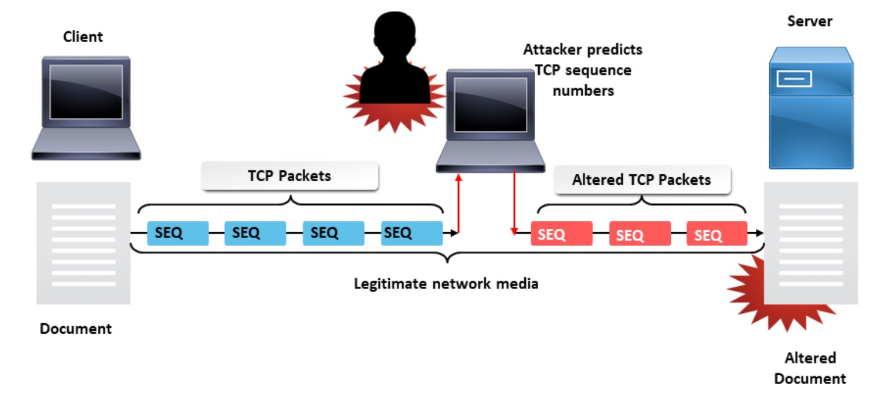
\includegraphics{./tex2pdf.-328d711c/36ac2e7821c194b1d375d23d12f30d45036e7277.png}
\caption{Untitled}
\end{figure}

\textbf{SYN Flooding Attack:}

An attacker sends a large number of SYN requests to a target's system.
The target then uses a lot of resources to attempt to process these
requests. Usually, SYN flood packets use spoofed source IP addresses,
and no TCP connection is ever established. It makes it very hard for the
target to work out which TCP SYN is a legitimate connection attempt.

\textbf{SYN Flooding Solutions:}

\begin{itemize}
\item
  Ingress Filtering - Routers install filters to drop packets from
  networks that are not downstream.
\item
  uRPF Checks - Accept packet from interface only if forwarding table
  entry for source IP matches ingress interface. If there are multiple
  routes between the client and server this check can no longer work as
  it may only show up in a few forwarding tables.
\item
  TCP SYN cookies - The client and server require SYN/ACK numbers to be
  as expected.
\end{itemize}

\textbf{IP Spoofing:}

The creation of fake packets with fake source IP addresses to
impersonate another computer. The hacker intercepts a TCP handshake
before the source manages to send its SYN-ACK message. Instead, the
hacker sends a fake confirmation including their device address (MAC)
and a spoofed IP address. It used generally used to bypass firewalls
that rely on blacklisting. It can also be used for DoS attacks using SYN
flooding attacks. IP spoofing is used in man-in-the-middle attacks to
pretend they are both the client and server.

\textbf{ARP: Address Resolution Protocol}

ARP Resolves IP addresses to MAC addresses. Each IP node on a LAN has an
ARP table (Host, Router). The ARP table is a mapping from IP addresses
to MAC addresses. It works by broadcasting and caching responses. The
protocol begins with a computer broadcasting a message of the form ``who
has \textless{}IP address 1\textgreater{} tell \textless{}IP address
2\textgreater{}'' when the machine with ``address 1'' receives the
message it broadcasts its MAC address back to ``address 2''.

\textbf{ARP Spoofing:}

\begin{itemize}
\item
  The ARP table is updated whenever an ARP response is received
\item
  Requests are not tracked, ARP announcements are not authenticated and
  machines trust each other.
\item
  ARP caches can be poisoned by sending fake ARP replies, ARP tables
  will update themselves even if they didn't send a request.
\end{itemize}

\textbf{Common types of DDoS attacks:}

\begin{itemize}
\item
  Application layer attacks - HTTP
\item
  Protocol Attacks - TCP (SYN Flooding)
\item
  Volumetric Attacks - DNS Amplification.
\end{itemize}

\end{document}
